\section{Problema 3: Girl Scouts}
\subsection{Descripción del problema}

En este ejercicio existe un grupo de niñas exploradoras, algunas de ellas amigas entre sí, que deben formarse en una ronda. Siendo $e$ la cantidad de exploradoras, existen $(e-1)!$ permutaciones posibles en las cuales pueden sentarse. Podemos medir la distancia entre dos amigas como la mínima cantidad de chicas que hay entre una y otra, más 1. Por ejemplo, si una chica está al lado de la otra, la distancia entre ellas es 1. Si tenemos una ronda de tres chicas, la distancia entre cualquier par de chicas va a ser 1.

El problema consiste en hallar la forma de ubicar a las exploradoras de forma tal que exista la menor distancia posible entre cada amistad, y logrando que la suma total de la distancia entre todos los pares de amigas sea mínima.

El formato de entrada es un archivo de texto que contiene una línea por cada grupo de exploradoras. Cada grupo de exploradoras es una instancia distinta del problema. Cada línea se compone de una sucesión de amistades separadas por \texttt{;} de la forma \texttt{amistad[;amistad]}. Cada amistad es un par \texttt{x xs} donde \texttt{x} es una letra y \texttt{xs} una cadena de letras.

Veamos un ejemplo. Tenemos un grupo de 5 chicas: A, B, C, D y E. A es amiga de B y C, y D es amiga de C. Esto se puede escribir de muchas maneras. Si escribimos a cada amistad dos veces, podemos hacerlo así:

\texttt{A BC;B A;C AD;D C;E}

Si las sentamos así:

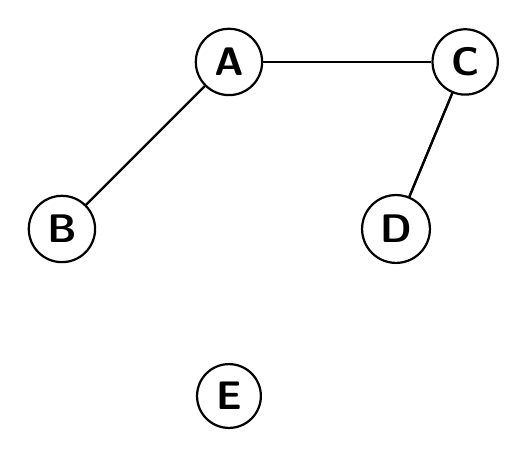
\begin{tikzpicture}[auto, node distance=3cm, every loop/.style={},
                    thick,main node/.style={circle,draw,font=\sffamily\Large\bfseries}]

  \node[main node] (1) {A};
  \node[main node] (2) [below left of=1] {B};
  \node[main node] (3) [below right of=2] {E};
  \node[main node] (4) [below right of=1] {D};
  \node[main node] (5) [right of=1] {C};

  \path[every node/.style={font=\sffamily\small}]
    (1) edge node [left] {} (2)
        edge node[right] {} (5)
    (2) edge node [right] {} (1)
    (4) edge node [left] {} (5)
    (5) edge node {} (4);
\end{tikzpicture}

vamos a estar obteniendo una solución óptima, ya que la suma total de distancias es 3 (contando a cada amistad una sola vez) y la distancia máxima es 1.

El formato de salida para cada grupo de exploradoras es una línea de texto donde se debe indicar la distancia máxima obtenida, seguida de un espacio y una cadena de letras que indica la forma en que fueron sentadas las exploradoras. En caso de haber obtenido más de una solución, se debe devolver la primera en órden alfabético. Para el último ejemplo, la forma de codificar sería así:

\texttt{1 ACDEB}

Nótese que es equivalente a esta otra: \texttt{1 CDEBA}, ya que la única diferencia es por cuál exploradora empezamos a describir la ronda.

%El algoritmo a implementar debe hallar, utilizando backtracking, la permutación en donde la separación entre las niñas que son amigas sea mínima. La técnica algorítmica para resolver el problema puede reducirse a una decisión simple en cada paso: para cada posicion, determinar a qué niña colocar. La mecánica del backtracking busca detectar las instancias en donde los resultados serán peores que el mejor caso registrado, independientemente de las decisiones que se tomen adelante en esa misma rama; de esta forma, se evita el computo de permutaciones que no resultarán óptimas.


\subsection{Algoritmo desarrollado}

Desarrollamos un algoritmo que utiliza la técnica de \textit{backtracking}. Esta técnica consiste en generar de forma incremental candidatos parciales para formar soluciones. De forma implícita, los candidatos parciales pueden ser representados como los nodos de un árbol; las soluciones completas son las hojas del árbol. El algoritmo va generando el árbol de forma recursiva al hacer un recorrido DFS. En cada paso, se hace una evaluación que permite decidir si las hojas descendientes del candidato parcial actual pueden ser solución o no del problema. De esta manera, se evalúa todo el árbol de posibilidades sin necesariamente recorrerlo entero, ya que se pueden descartar ramas enteras antes de entrar en ellas.

Aplicando esta técnica a este problema en particular, desarrollamos un algoritmo de \textit{backtracking} que busca las mejores permutaciones posibles para las niñas exploradoras. El algoritmo comienza con una ronda vacía con tantos lugares como exploradoras hay en el grupo. Los lugares son fijos, y medimos la distancia entre dos chicas como la cantidad de lugares que me tengo que ``mover'' para llegar de una chica a la otra.

Separamos a las exploradoras en dos grupos: aquellas que no tienen ninguna amiga, y aquellas que sí (tienen al menos una amistad). A las que no tienen amigas las ubicaremos en la ronda solamente al final, ya que, una vez ubicadas todas las exploradoras que sí tienen amigas, aquellas que no tienen amistades no influirán en las distancias, y cualquier permuitación de las chicas sin amigas será equivalente en el resultado final (podemos simplemente generar la que es alfabéticamente primera, descartando las otras).

En cada paso del algoritmo recursivo vamos agregando una chica a la ronda en un lugar determinado (que queda fijo), sin modificar la ubicación de las que ya están en la ronda. Luego, evaluamos si la distancia máxima entre pares de amigas es mayor a la mejor obtenida (para alguna solución óptima hallada anteriormente). Si lo es, entonces descartamos todas las ramas que descienden de este caso y retornamos, de manera tal de continuar la ejecución por otra rama del árbol. Si no lo es, continuamos la exploración del árbol, a menos que ya hayamos llegado a una hoja. En tal caso, si la solución obtenida es mejor a la que hasta ahora era la mejor, la nueva solución pasa a ser la mejor. Al finalizar el recorrido completo, se devuelve la solución que fue guardada como la mejor.

Para medir la sumatoria de distancias entre pares de amigas en cada iteración no es necesario recalcular todas las distancias en la ronda. Simplemente se deben calcular las distancias de la exploradora que se agrega con sus amigas que ya esten ubicadas.



\subsection{Justificación de correctitud}

El hecho de estar generando todo el árbol de posibilidades nos asegura no estar dejando fuera soluciones posibles. El cuidado debe estar, entonces, en realizar las podas de forma correcta y de medir distancias de forma correcta. Analicemos más en detalle las podas realizadas:

\begin{itemize}
 \item Una vez ubicadas todas las exploradoras que tienen amigas, no probamos las distintas combinaciones con aquellas exploradoras que no tienen amigas: simplemente elegimos la permutación que está primera alfabéticamente. Esto es correcto ya que las exploradoras que no tienen amigas no forman parte de ninguna amistad, con lo cual, no cambian en nada a las distancias.
 \item A medida que se van formando los distintos fogones, se chequea en cada instancia si el caso que se está construyendo produce una mayor separación promedio que el mejor caso registrado. Es decir, si en un fogón, aún estando incompleto, se registra mayor separación entre amigas, se concluye que todas las posibles permutaciones que partan desde ese punto no seran óptimas.
 \end{itemize}
 
\subsection{Análisis de la complejidad temporal}
La cantidad de posibles permutaciones para una ronda es de $(e-1)!$; en el peor escenario posible, los datos de entradas tienen un orden tal que el algoritmo encuentre una mejor situación en cada iteración, por lo cual tendrá que recorrer las $(e-1)!$ permutaciones.

Cada permutación del fogon cuesta no más de $2*e$ pasos. En cada paso, al colocar o quitar una exploradora, se debe calcular la alteración que se produce en la distancia de amistades. Para esto se debe chequear para cada amiga de la exploradora si ésta está en el fogon y, en caso afirmativo, cuál es su posición. Lógicamente, la cantidad de amistades de una exploradora está acotada por $a$ y, como se utiliza un \texttt{TreeMap} para identificar las posiciones de las exploradoras con amigas, determinar la posicion de cada amiga en el fogón puede resolverse en $ln a$

En un peor caso, entonces, la complejidad del algoritmo pertenece a $O( (e-1)! \cdot e \cdot a \cdot \log{}a)$ lo cual está acotado por $O(e^e \cdot a \cdot \log{}a)$, estrictamente menor a la complejidad solicitada en el enunciado.

%\subsection{Tests de correctitud}


\subsection{Experimentación para observar la performance real}

%\subsubsection{Peor caso}

%\subsubsection{Caso promedio}

Se generaron casos de test de forma aleatoria, dejando fijo el valor de e (en 10), e incrementando el valor de a. El valor máximo de a es la mitad de $e (e-1)$, ya que no es posible tener más amistades. La relación entre el tiempo de ejecución y $a$, en este caso, se puede ver en los gráficos \ref{Efijot} y \ref{Efijotdividido}.

 \begin{figure}[h!]
   \begin{center}
 	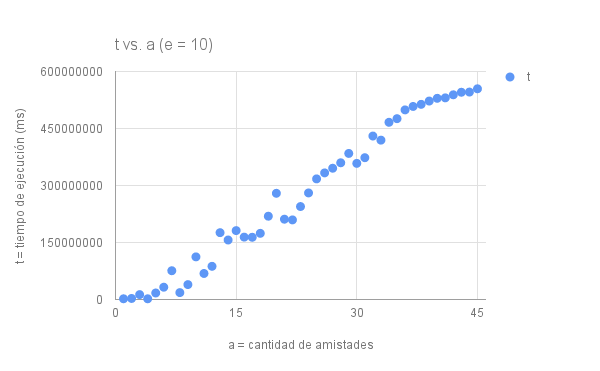
\includegraphics[width=11cm]{imagenes/ej3/Efijo-t.png}
	\caption{e = 10. Relación entre tiempo de ejecución y cantidad de amistades.}
	\label{Efijot}
   \end{center}
 \end{figure}
 
 \begin{figure}[h!]
   \begin{center}
 	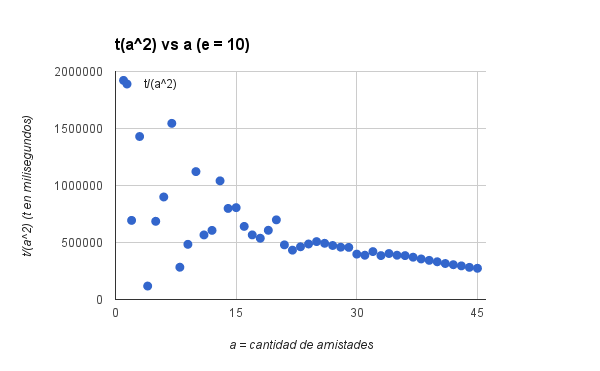
\includegraphics[width=11cm]{imagenes/ej3/Efijo-tdividido.png}
	\caption{e = 10. Relación entre tiempo de ejecución y cantidad de amistades. Dividimos el tiempo por $a^2$.}
	\label{Efijotdividido}
   \end{center}
 \end{figure}

En el gráfico \ref{Efijotdividido} se puede apreciar que la curva tiende a cero. Esto implica que la curva de tiempos está acotada por la curva de $a^2$.


Se generaron también tests de forma aleatoria dejando el valor de $a$ fijo en relación a $e$ de manera tal que $a = e$ y se obtuvieron los siguientes gráficos de performance (\ref{EAt} y \ref{EAtdividido}).

 \begin{figure}[h!]
   \begin{center}
 	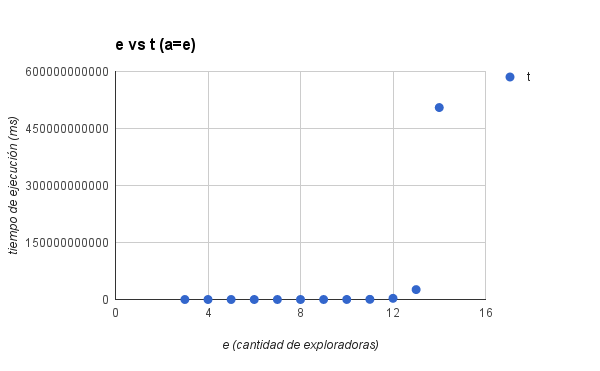
\includegraphics[width=11cm]{imagenes/ej3/EA-t.png}
	\caption{Relación entre tiempo de ejecución y cantidad de exploradoras ($a=e$).}
	\label{EAt}
   \end{center}
 \end{figure}
 
 \begin{figure}[h!]
   \begin{center}
 	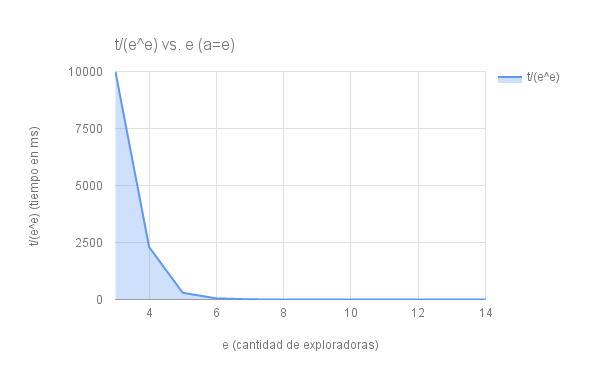
\includegraphics[width=11cm]{imagenes/ej3/EA-tdividido.png}
	\caption{Relación entre tiempo de ejecución y cantidad de exploradoras ($a=e$). Dividimos el tiempo por $e^e$.}
	\label{EAtdividido}
   \end{center}
 \end{figure}
 
 Nuevamente, en el gráfico \ref{EAtdividido} se puede ver cómo la curva tiende a cero, con lo cual podemos decir que también el tiempo de ejecución está acotado por $e^e$.
 
 De estos análisis, podemos concluir que empíricamente el algoritmo implementado cumple con las cotas de complejidad, al menos para casos promedio, de ser $O(e^e a^2)$.
 
 \subsection{Código fuente}
A continuación se incluyen las partes más relevantes del código.\\

\lstinputlisting[name=Solucion, numbers=left, frame=lines, firstline=8, lastline=203]{../src/ej3/ej3/src/Solucion.java}
%Los métodos que manipulan los heaps que se encuentran en la clase \emph{Heap.java}
%\lstinputlisting[name=Heaps, numbers=left, frame=lines, firstline=7, lastline=18]{../src/ej2/src/Heap.java}
%\lstinputlisting[name=Heaps, numbers=left, frame=lines, firstline=20, lastline=38]{../src/ej2/src/Heap.java}
%\lstinputlisting[name=Heaps, numbers=left, frame=lines, firstline=40, lastline=52]{../src/ej2/src/Heap.java}